\documentclass[11pt,a4paper]{article}
\usepackage[a4paper,margin=2.6cm]{geometry}
\usepackage{iftex}
\ifPDFTeX
  \usepackage[T2A]{fontenc}
  \usepackage[utf8]{inputenc}
  \usepackage[russian]{babel}
\else
  \usepackage{fontspec}
  \usepackage{polyglossia}
  \setdefaultlanguage{russian}
  \setotherlanguage{english}
  \defaultfontfeatures{Ligatures=TeX}
  \setmainfont{Times New Roman}
  \setsansfont{Arial}
  \setmonofont{Courier New}
  \newfontfamily\cyrillicfont{Times New Roman}
  \newfontfamily\cyrillicfontsf{Arial}
  \newfontfamily\cyrillicfonttt{Courier New}
\fi
\usepackage{microtype}
\usepackage{mathtools,amssymb}
\usepackage{graphicx}
\usepackage{booktabs}
\usepackage{float}
\usepackage{caption}
\captionsetup{font=small,labelfont=bf}
\usepackage{enumitem}
\setlist{nosep,leftmargin=1.5em}
\usepackage{csquotes}
\usepackage{tikz}
\usetikzlibrary{arrows.meta,positioning}
\usepackage[backend=biber,style=numeric-comp,sorting=none,maxbibnames=6]{biblatex}
\addbibresource{references_v2.bib}
\usepackage[unicode,hidelinks]{hyperref}
\setlength{\emergencystretch}{2em}

\title{Инвариант сопряжённости масштабов как проекция квазинеизменной\\
организации атмосферной циркуляции:\\
теоретическая рамка и районирование}
\author{Сотириади Н.}
\date{2026}

\begin{document}
\maketitle

\begin{abstract}
Локальная организация атмосферной циркуляции определяется большим числом сосуществующих факторов --- орографией, распределением суши и океана, климатологией конвективной неустойчивости, интенсивностью синоптической вихревой активности, режимом межгодовой изменчивости, --- совместно образующих многомерное поле квазинеизменных на наблюдаемом отрезке условий $\theta(x)$. В первых двух статьях серии показано, что скалярный профиль сопряжённости соседних октавных уровней $P(x)$ --- устойчивый, воспроизводимый в независимых реанализах и в расчёте без усвоения наблюдений, статистически атрибутируемый региональный инвариант. Настоящая, завершающая работа серии даёт этой величине интерпретирующую рамку: $P(x)=\Phi[\mu_{\theta(x)}]$ --- функционал инвариантной меры быстрой (часы) динамики при квенчированном (устойчивом на десятилетия и дольше) поле условий $\theta(x)$, а не переменная какой-либо динамической системы. Из рамки выведено и проверено её единственное содержательное следствие: статичный функционал сложившегося режима не должен опережать перестройку режима и превосходить по чувствительности стандартные показатели --- проверка на переходе 1998/99~гг. подтверждает это следствие. Отдельно предъявлен завершённый аудит новизны конструкции: форма оценки (сопряжённость соседних огибающих) не нова --- её ближайшие формальные родственники суть корреляция амплитудных огибающих в нейрофизиологии и коэффициент амплитудной модуляции в турбулентности, а рангово-копульная составляющая конструкции декоративна ($\rho=0{,}99$ с линейным аналогом); новизна состоит в свойствах объекта --- заякоренная сверхспектральная компонента является устойчивым, физически атрибутируемым, низкоразмерным (одна ведущая ось --- 85\,\% качества предсказания) картируемым инвариантом. Основной прикладной тезис: именно низкая эффективная размерность делает скаляр $P$ полезной осью районирования --- он сжимает многомерное пространство локальных условий в одну сопоставимую по территориям координату, сохраняя воспроизводимую (потолок $R^2=0{,}91$), лишь частично объяснённую (до 83\,\% на сегодняшнем наборе признаков) и несводимую к шуму остаточную географию, отнесённую к дальнейшей работе. Статья не выходит за пределы уже выполненных проверок и не делает предсказательных выводов.

\smallskip
\noindent\textbf{Ключевые слова:} квенчированные условия, инвариантная мера, районирование, эффективная размерность, атмосферная циркуляция, региональный инвариант, реанализ.
\end{abstract}

\section{Постановка}
\label{sec:intro}

Две первые статьи серии\footnote{Сотириади~Н. Сопряжённость иерархических уровней атмосферной циркуляции как региональный инвариант; Глобальная география сопряжённости иерархических уровней атмосферной циркуляции: атрибуция и планетарная карта (первая и вторая статьи настоящей серии). Протоколы, код и численные результаты всех трёх работ открыты в едином репозитории: \url{https://github.com/Theclimateguy/Shroedinger}.} решили две эмпирические задачи: профиль сопряжённости соседних октавных уровней~$P$ построен и проверен на статус регионального инварианта (статья~I), его глобальная география закартирована и статистически атрибутирована (статья~II). Возникает законный вопрос: какую роль в исследовательской программе играет теоретическая интерпретация, если она не добавляет ни новых данных, ни новых проверок?

Ответ определяет структуру статьи. Интерпретация нужна не для предсказания, а для трёх вещей. Во-первых, для честной постановки вопроса о новизне: конструкция <<корреляция огибающих соседних масштабных полос>> существует в нескольких дисциплинах, и без прямого, заранее регламентированного сопоставления с претендентами на приоритет любое утверждение о новизне уязвимо (разд.~\ref{sec:audit}). Во-вторых, для точной формулировки того, что означает <<один скаляр как инвариант>> в терминах статики и динамики системы --- какие утверждения при этом делаются, а какие принципиально не делаются (разд.~\ref{sec:frame}). В-третьих, для обоснования конкретного прикладного тезиса: использования~$P$ как оси районирования, сжимающей многомерное пространство локальных условий (разд.~\ref{sec:zoning}).

Существенно разграничение с исходной, более амбициозной постановкой программы. На старте предполагалось, что сопряжение уровней циркуляции может быть \emph{активной, динамически изменяющейся связью} между масштабами --- что один масштаб может <<вести>> другой, а сила связи --- предсказуемо эволюционировать. Более двадцати преднамеренно фальсификационных проверок программы (включая четыре завершающих аудита) показали обратное: связь статична. Это не потеря результата, а содержательный вывод, который разд.~\ref{sec:frame} формулирует явно и без потери фальсифицируемости.

\section{Материал и метод}
\label{sec:data}

Полное описание данных, построения дескриптора и всех протоколов дано в статьях~I--II и здесь не повторяется. Все числовые результаты настоящей статьи заимствованы из уже завершённых и замороженных протоколов; новых расчётов статья не выполняет.

Единственное методическое уточнение, специфичное для настоящей работы: рангово-копульная составляющая определения~$P$ --- использование ранговой, а не линейной корреляции огибающих --- является декоративным элементом конструкции, не несущим самостоятельной информации (разд.~\ref{sec:audit}, строка~3 табл.~\ref{tab:audit}). Поэтому здесь определение приводится без апелляции к <<копуле>> как содержательному ингредиенту: $P$ --- корреляция логарифмов карт активности соседних октавных полос поля относительного вихря на 850~гПа \cite{Hersbach2020,Soci2024}, взятая в превышении над медианой ансамбля фазовых суррогатов (заякоренная, сверхспектральная форма); выбор ранговой реализации --- техническая деталь.

\section{Аудит новизны: чем $P$ не является}
\label{sec:audit}

Раздел строится как прямой ответ на ожидаемое возражение <<это известная статистика с новым именем>> --- и снимает его предъявлением завершённого, заранее зафиксированного аудита, а не декларацией. Для каждого претендента на приоритет до вычислений были заморожены порог тождества (ранговая корреляция карт двух статистик $0{,}90$) и порог родственности ($0{,}60$); сопоставление велось на общем носителе (902 глобальных тайла статьи~II) и продублировано на укрупнённом носителе (24 единицы: 12 равновеликих областей $\times$ 2 окна разных лет и сезонов, полная лестница полос до 1600~км). Итоги --- в табл.~\ref{tab:audit}.

\begin{table}[t]
\centering
\caption{Аудит новизны конструкции $P$: сопоставление с претендентами на приоритет. Порог тождества $\rho=0{,}90$, порог родственности $0{,}60$; заморожены до вычислений.}
\label{tab:audit}
\small
\begin{tabular}{@{}p{0.30\linewidth}p{0.36\linewidth}p{0.24\linewidth}@{}}
\toprule
Претендент & Проверка & Итог\\
\midrule
Коэффициент амплитудной модуляции турбулентности \cite{Mathis2009} & $\rho(P,R_{\mathrm{AM}})=+0{,}14$ на 902 тайлах; $+0{,}39$ на 24 областях & не тождественны; форма родственна, объект различен\\
Логнормальный каскад Колмогорова--Обухова, мультифрактальный формализм \cite{LovejoySchertzer2013} & $\rho(P,P_{\mathrm{casc}})=-0{,}42$ (тайлы), $+0{,}04$ (области); каскадное предсказание --- спектральная величина: его заякоренная компонента $\approx0$, у $P$ --- $0{,}26$ & различие устойчиво на обоих масштабах\\
Ранг/копула как содержательный ингредиент & $\rho(P,P_{\mathrm{lin}})=+0{,}99$ (тайлы), $+0{,}98$ (области); на непересекающихся половинах выборки $+0{,}89$ ($\approx0{,}98$ после коррекции на затухание) & ингредиент декоративен; копульный язык снят со всех трёх статей\\
Логарифмическая дисперсия огибающей (параметр интермиттентности) & $\rho(P,\sigma^2_{\ln E})=+0{,}69$ на тайлах (шумоустойчивая оценка $+0{,}60$); $+0{,}92$ на 24 областях & содержательный, но не тождественный родственник; усиление связи с масштабом --- открытый пункт (см. текст)\\
\bottomrule
\end{tabular}
\end{table}

Итог аудита формулируется для печати так. Сопряжённость соседних огибающих масштабных полос --- \emph{известная} конструкция; её ближайшие формальные родственники --- корреляция амплитудных огибающих частотных полос в нейрофизиологии \cite{Bruns2000} (в составе более широкой литературы о межчастотной связи \cite{Canolty2006}) и коэффициент амплитудной модуляции пристеночной турбулентности \cite{Mathis2009}. Недавняя критика последнего как величины, отчасти наследующей спектральные и фазовые свойства поля \cite{CuiJacobi2025}, указывает ровно на тот дефект, который в статьях~I--II устраняется анкорированием на фазовых суррогатах, и тем самым поддерживает принятое там методическое решение. Новизна работы --- не в оценивающей статистике и не в её названии, а в демонстрации того, что заякоренная, сверхспектральная компонента этой известной конструкции является устойчивым региональным инвариантом атмосферной циркуляции: картируемым глобально, воспроизводимым в расчёте без усвоения наблюдений и физически атрибутируемым, --- то есть в свойствах \emph{объекта}, а не в свойствах оценки.

Две оговорки фиксируются явно. Первая: связь $P$ с параметром интермиттентности (дисперсией логарифма огибающей) зависит от масштаба носителя --- $+0{,}60$--$0{,}69$ на тайлах против $+0{,}92$ на укрупнённых областях; величина на областях получена как сопровождающая (не замороженная как основная) оценка на $n=24$ со стандартной ошибкой около $0{,}2$ и потому сообщается как открытый пункт, требующий отдельного протокола, а не как результат. Вторая: вопрос о сведении $P$ к стандартным характеристикам инвариантной меры (локальная размерность, экстремальный индекс, спектр оператора переноса) содержателен --- предварительный пилот дал $\rho(P,d)\approx+0{,}5$ на 48 оконных выборках, --- но его статус --- черновой, незамороженный протокол; в настоящей серии он числится открытым направлением (разд.~\ref{sec:bounds}) и как решённый нигде не используется.

\section{Теоретическая рамка: статичная характеристика устоявшегося режима}
\label{sec:frame}

Раздел вводит интерпретирующий язык на основе уже выполненных проверок; каждый новый символ определяется явно, и ни одно утверждение не выходит за пределы измеренного. Схема рамки --- на рис.~\ref{fig:scheme}.

\begin{figure}[t]
\centering
\begin{tikzpicture}[
  box/.style={draw, rounded corners=2pt, align=left, inner sep=7pt,
              text width=0.62\linewidth, font=\small},
  side/.style={align=left, text width=0.26\linewidth, font=\footnotesize},
  arr/.style={-{Latex[length=2.5mm]}, thick},
  node distance=9mm]
\node[box] (theta) {\textbf{Квазинеизменное поле условий $\theta(x)$}\\[2pt]
ярус 1 --- экзогенные граничные условия: орография, суша/океан, инсоляция, распределение ТПО;\\
вместе с закреплённой ими стационарной организацией циркуляции (штормовые пути, очаги конвекции).\\[2pt]
Измеренная нижняя граница времени изменения: $T_\theta\gg46$~лет};
\node[box, below=of theta] (mu) {\textbf{Быстрый слой: $\omega_t(x)$ --- относительный вихрь на 850~гПа}\\[2pt]
стохастическая эволюция с перемешиванием $T_{\mathrm{fast}}\approx9$--$11$~ч, единым для всех полос 71--1131~км ($\alpha=0{,}00$; 95-\%-й интервал $[-0{,}08;+0{,}11]$);\\
локально эргодичен на инвариантной мере $\mu_{\theta(x)}$};
\node[box, below=of mu] (P) {\textbf{Наблюдаемая: $P(x)=\Phi[\mu_{\theta(x)}]$}\\[2pt]
статичная сверхспектральная проекция меры; собственной динамики не имеет --- колеблются лишь выборочные оценки, декоррелирующие на такте перемешивания выборки ($\sim$10~ч)};
\draw[arr] (theta) -- node[right=2mm, font=\footnotesize\itshape]{задаёт параметры быстрой динамики} (mu);
\draw[arr] (mu) -- node[right=2mm, font=\footnotesize\itshape]{функционал меры, а не состояния} (P);
\node[side, right=4mm of theta.north east, anchor=north west] {ярус 1: допустим направленный язык (<<формирует>>)};
\node[side, right=4mm of P.north east, anchor=north west] {ярус 2 (CAPE, синоптическая вихревая энергия): совместное формирование с $P$, пик связи на нулевом сдвиге, без опережения};
\end{tikzpicture}
\caption{Рамка квазинеизменной организации: поле условий $\theta(x)$, квенчированное на отрезке наблюдения, задаёт инвариантную меру быстрого слоя $\mu_{\theta(x)}$; наблюдаемая $P(x)$ --- статичный функционал этой меры. Все указанные числа --- измеренные величины из статей I--II и протоколов программы.}
\label{fig:scheme}
\end{figure}

\subsection{Быстрый и медленный (квазинеизменный) слои}
\label{sec:layers}

Разрешённое состояние атмосферы $\omega_t(x)$ --- в инструментах программы относительный вихрь на 850~гПа --- эволюционирует как быстрый стохастический процесс. Его время перемешивания измерено и составляет $T_{\mathrm{fast}}\approx9$--$11$~ч, причём оно \emph{не зависит от масштабной полосы}: показатель масштабной зависимости времени декорреляции по полосам 71--1131~км равен $\alpha=0{,}00$ при 95-\%-м интервале $[-0{,}08;+0{,}11]$ --- один такт, общий для всех разрешённых масштабов, тогда как вихревое время оборота дало бы шестикратный, а адвективное перемешивание --- одиннадцатикратный разброс.

Параметры этого процесса задаются полем условий $\theta(x)$: экзогенными граничными условиями (орография, конфигурация суши и океана, инсоляция, распределение температуры поверхности океана) вместе с закреплённой ими стационарной организацией циркуляции --- штормовыми путями и очагами конвекции. На отрезке наблюдения поле $\theta$ квенчировано --- заморожено в смысле статистической физики неупорядоченных систем: измеренная нижняя граница времени его изменения $T_\theta\gg46$~лет (устойчивость региональных статистик $P$ между полупериодами записи 1979--1997 и 1998--2016~гг. при тридцатикратном превышении статистической мощности относительно первоначальной проверки). Разрыв двух шкал --- десять часов против полувека --- и есть основание рассматривать слои раздельно.

\subsection{Наблюдаемая как функционал инвариантной меры}
\label{sec:functional}

При квенчированном $\theta(x)$ быстрый слой локально эргодичен на своей инвариантной мере $\mu_{\theta(x)}$. Наблюдаемая программы есть
\begin{equation}
P(x)=\Phi\!\left[\mu_{\theta(x)}\right],
\label{eq:phi}
\end{equation}
где функционал $\Phi$ выделяет ту часть меры, которая не фиксирована ни спектром вторых моментов, ни иерархией скаттеринг-моментов, ни каскадным предсказанием по дисперсиям логарифмов огибающих (разд.~\ref{sec:audit}) --- сверхспектральную текстуру сопряжения масштабов.

Ключевое утверждение рамки --- не гипотеза, а сводка установленного: \emph{функционал стационарной меры не имеет собственной динамики}. Колеблются только выборочные оценки $\Phi$, и декоррелируют они на времени перемешивания выборки --- том же $\sim$10-часовом такте, общем для всех полос, --- а не на каком-либо каскадном или иерархическом времени. Это следствие проверено трижды, независимыми методами и с преднамеренно фальсификационной постановкой каждый раз: (i)~релаксация $P$ к фиксированному региональному значению --- быстрая ($\sim$12~ч), без переносимой между регионами режимной зависимости; (ii)~отсутствие иерархии времён затухания по полосам (плоская $\tau_b(\ell)$, см. выше); (iii)~тождество для любого оценщика <<производной>> вида скользящего размаха разностей,
\begin{equation}
\operatorname{RMS}\!\left(X_t-X_{t-\delta}\right)=\sigma_X\sqrt{2\bigl(1-\rho_X(\delta)\bigr)},
\label{eq:rms}
\end{equation}
показывающее, что весь этот класс оценок является точной функцией амплитуды и персистентности ряда и не содержит третьей степени свободы --- то есть в принципе не может нести самостоятельного динамического содержания. Отрицательный результат при равной статистической мощности получен во всех трёх случаях; на нём, а не на постулате, держится статика рамки.

\subsection{Что означает <<отсутствие динамики>> на практике}
\label{sec:nodyn}

На старте программы всерьёз рассматривалась возможность, что сопряжение уровней --- активный, изменяющийся во времени процесс: что один масштаб опережает другой или что сила связи предсказуемо растёт и убывает. Проверки предыдущего пункта закрыли этот вопрос отрицательным результатом: измеримой активной связи такого рода на доступных временных масштабах нет. Это не пробел, а содержательный итог программы. Именно он обосновывает интерпретацию $P$ как статичной, а не эволюционирующей характеристики --- и именно на нём строится довод о применимости величины к районированию, а не к прогнозу (разд.~\ref{sec:zoning}, \ref{sec:bounds}).

\subsection{Причинная структура и координаты текстуры}
\label{sec:tiers}

Внутри организации различаются два яруса, и различие зафиксировано протоколом атрибуции \emph{до} вычислений. Для яруса~1 --- экзогенных граничных условий (орография, суша/океан, широта, градиент температуры поверхности океана) --- допустим направленный язык: они \emph{формируют} географию $P$. Для яруса~2 --- совместно складывающихся характеристик состояния (конвективный режим, синоптическая вихревая активность) --- направленный язык не используется: их связь с $P$ пикирует на нулевом временном сдвиге без опережения в какую-либо сторону, и корректное слово --- совместное формирование.

Эмпирически две координаты яруса~2 задают текстуру (статья~II): конвективный режим \emph{понижает} $P$ сверх того, что отражает спектр, --- интермиттентная, локально порождаемая завихренность конвективных режимов расцепляет соседние полосы; штормовая активность \emph{повышает} $P$ через тот же механизм, который формирует спектр, --- организованные бароклинные каскады выстраивают огибающие согласованно. Орография нагружает наклон спектра, а не $P$: две мишени управляются разными наборами условий.

\section{Районирование: одна скалярная ось на месте многомерного пространства условий}
\label{sec:zoning}

\subsection{Тезис}

Поле условий $\theta(x)$ по построению многомерно: восемь замороженных ковариат атрибуции (средняя высота и стандартное отклонение орографии, доля суши, дисперсия береговой линии, модуль широты, градиент температуры поверхности океана, климатология CAPE, синоптическая вихревая энергия) плюс четыре статистики интермиттентности огибающих --- не менее одиннадцати потенциально независимых осей описания локального режима. Скаляр $P(x)$ --- устойчивая и физически атрибутируемая проекция этого пространства на одну ось; при этом сама проекция эффективно \emph{одномерна} в сильном смысле: одна ковариата (синоптическая вихревая энергия штормовых путей) в одиночку даёт 85\,\% достижимого качества предсказания географии $P$ ($k_{80}=1$ при заранее заявленном пороге $\le3$; глобальный тайловый носитель статьи~II). В этом и состоит операциональное содержание тезиса <<большое пространство условий в одном скаляре>>: не в том, что многомерность иллюзорна, а в том, что для целей районирования --- ранжирования и классификации территорий по архитектуре сопряжения масштабов --- почти вся дискриминирующая способность многомерного $\theta$ извлекается одной осью, вычисляемой без каких-либо ковариат, из одного лишь поля вихря.

\subsection{Декомпозиция объяснённой дисперсии}

Ключевая количественная сводка раздела --- декомпозиция воспроизводимой дисперсии глобальной карты (табл.~\ref{tab:decomp}, рис.~\ref{fig:decomp}). Потолок надёжности карты --- $R^2=0{,}914$ по внутрисезонному расщеплению выборки пополам с поправкой Спирмена--Брауна; подчеркнём, что более ранняя межсезонная оценка ($0{,}603$) занижала потолок, списывая реальное сезонное изменение карты на шум, и во всех статьях серии заменена внутрисезонной.

\begin{table}[t]
\centering
\caption{Декомпозиция воспроизводимой дисперсии глобальной карты $P$ (902 тайла). Доли отнесены к потолку надёжности $R^2=0{,}914$.}
\label{tab:decomp}
\small
\begin{tabular}{@{}p{0.56\linewidth}p{0.38\linewidth}@{}}
\toprule
Компонента & Доля от потолка\\
\midrule
Восемь ковариат атрибуции (ведущая ось --- синоптическая вихревая энергия) & 59\,\% ($R^2=0{,}536$)\\
$+$ блок статистик интермиттентности & 83\,\% (декоррелированный прирост $+0{,}207$; $p=0{,}001$)\\
Остаток: воспроизводимый, не спектральный, географически организованный & $\approx15$\,\% (воспроизводимость $r=0{,}64$ при пороге $0{,}30$)\\
Невоспроизводимая часть (собственно шум оценки) & $\approx9$\,\% ($1-0{,}914$)\\
\bottomrule
\end{tabular}
\end{table}

\begin{figure}[t]
\centering
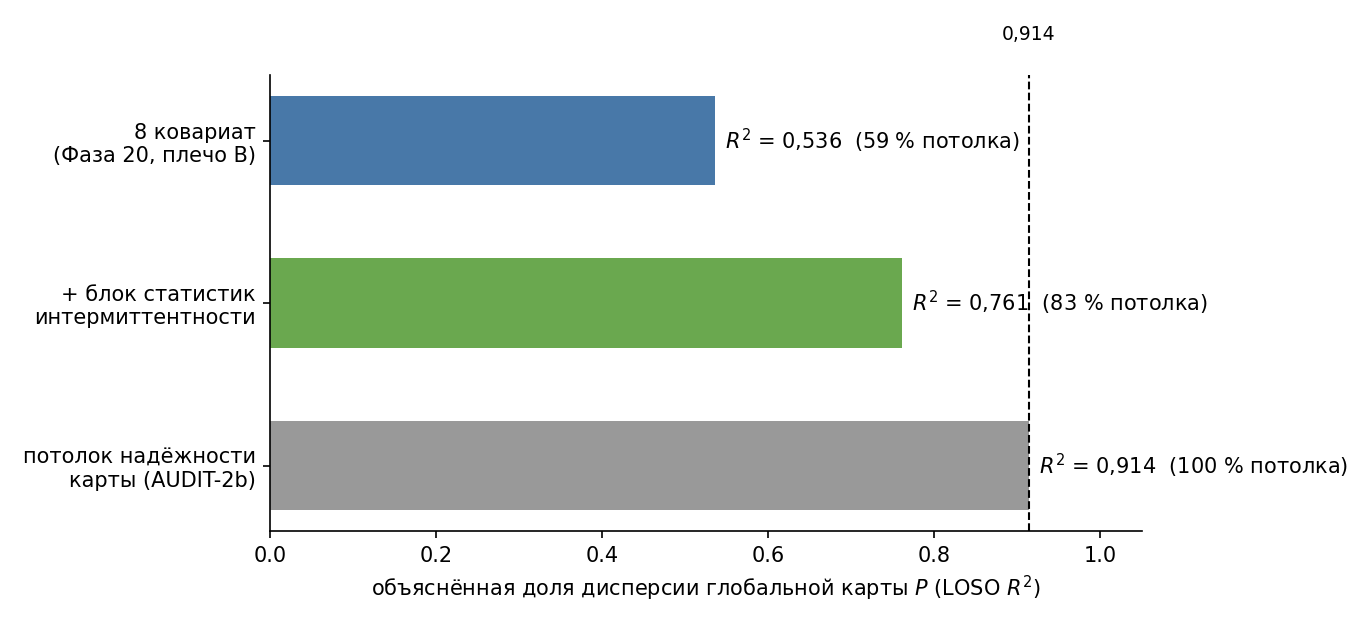
\includegraphics[width=0.82\linewidth]{figures/fig3_decomposition.png}
\caption{Декомпозиция объяснённой дисперсии глобальной карты $P$: восемь ковариат атрибуции (59\,\% потолка), с добавлением блока статистик интермиттентности (83\,\%) и потолок надёжности карты по внутрисезонному расщеплению выборки пополам ($R^2=0{,}914$, штриховая линия).}
\label{fig:decomp}
\end{figure}

\subsection{Почему это полезно для районирования, а не для предсказания}

Инвариант, лишённый собственной динамики (разд.~\ref{sec:frame}), не подходит для задач, требующих предвидеть изменение режима, --- и не должен для них использоваться: это прямо проверено и подтверждено на переходе 1998/99~гг. (разд.~\ref{sec:bounds}). Но именно отсутствие динамики делает величину надёжной осью \emph{статической} классификации территорий: она не дрейфует на операционных горизонтах; воспроизводится независимо от инструмента --- в другом реанализе и в модели без усвоения наблюдений; и не получается простой регрессией на стандартные метеорологические поля --- около 15\,\% её воспроизводимой дисперсии физичны и не редуцируются имеющимся набором признаков. Практический вывод: $P$ пригоден как дополнительная, дёшево вычисляемая координата районирования территорий по архитектуре мультимасштабного сопряжения --- рядом с показателями штормовой активности и конвективного режима, а не вместо них; его ценность --- не новая физика, а компактная, сопоставимая по территориям сводка многомерных локальных условий в одном числе. Тем самым линия инвариантов организации территории \cite{Puzachenko1986,Puzachenko2004,Puzachenko2010,Krenke2019} продолжается на новом уровне: от выделения иерархических уровней --- к измерению их отношения и к использованию этого отношения как координаты районирования.

\subsection{Остаточная география: задел, а не результат}

Необъяснённые $\approx$15\,\% воспроизводимой дисперсии карты --- не шум (рис.~\ref{fig:residual}): остаток воспроизводится между независимыми половинами выборки ($r=0{,}64$ против порога решающего правила $0{,}30$), не является спектральной величиной (связь с наклоном спектра и логарифмическими дисперсиями полос не превышает $0{,}12$ по модулю) и имеет распознаваемую географию. Отрицательные доли --- муссонные окраины и склоны крупной орографии: юго-восток Китая, боливийское и аргентинское предгорья, мексиканское плато, запад Аравии, Иран, Адриатика; положительные --- очаги глубокой конвекции и высокоширотные окраины суши: бассейн Конго, северо-запад Амазонии, Новая Гвинея, долина Ганга, Лабрадор, Гудзонов залив. Поскольку тайлы со средней высотой более 1200~м исключены из карты по замороженному правилу, а часть отрицательных долей лежит непосредственно у границы исключения, естественная первая гипотеза --- неразрешённый орографический член; она названа здесь как гипотеза для будущей работы и в настоящей серии не проверяется: протокол завершающего аудита содержал явный запрет на подбор ковариат под остаток внутри самого аудита.

\begin{figure}[t]
\centering
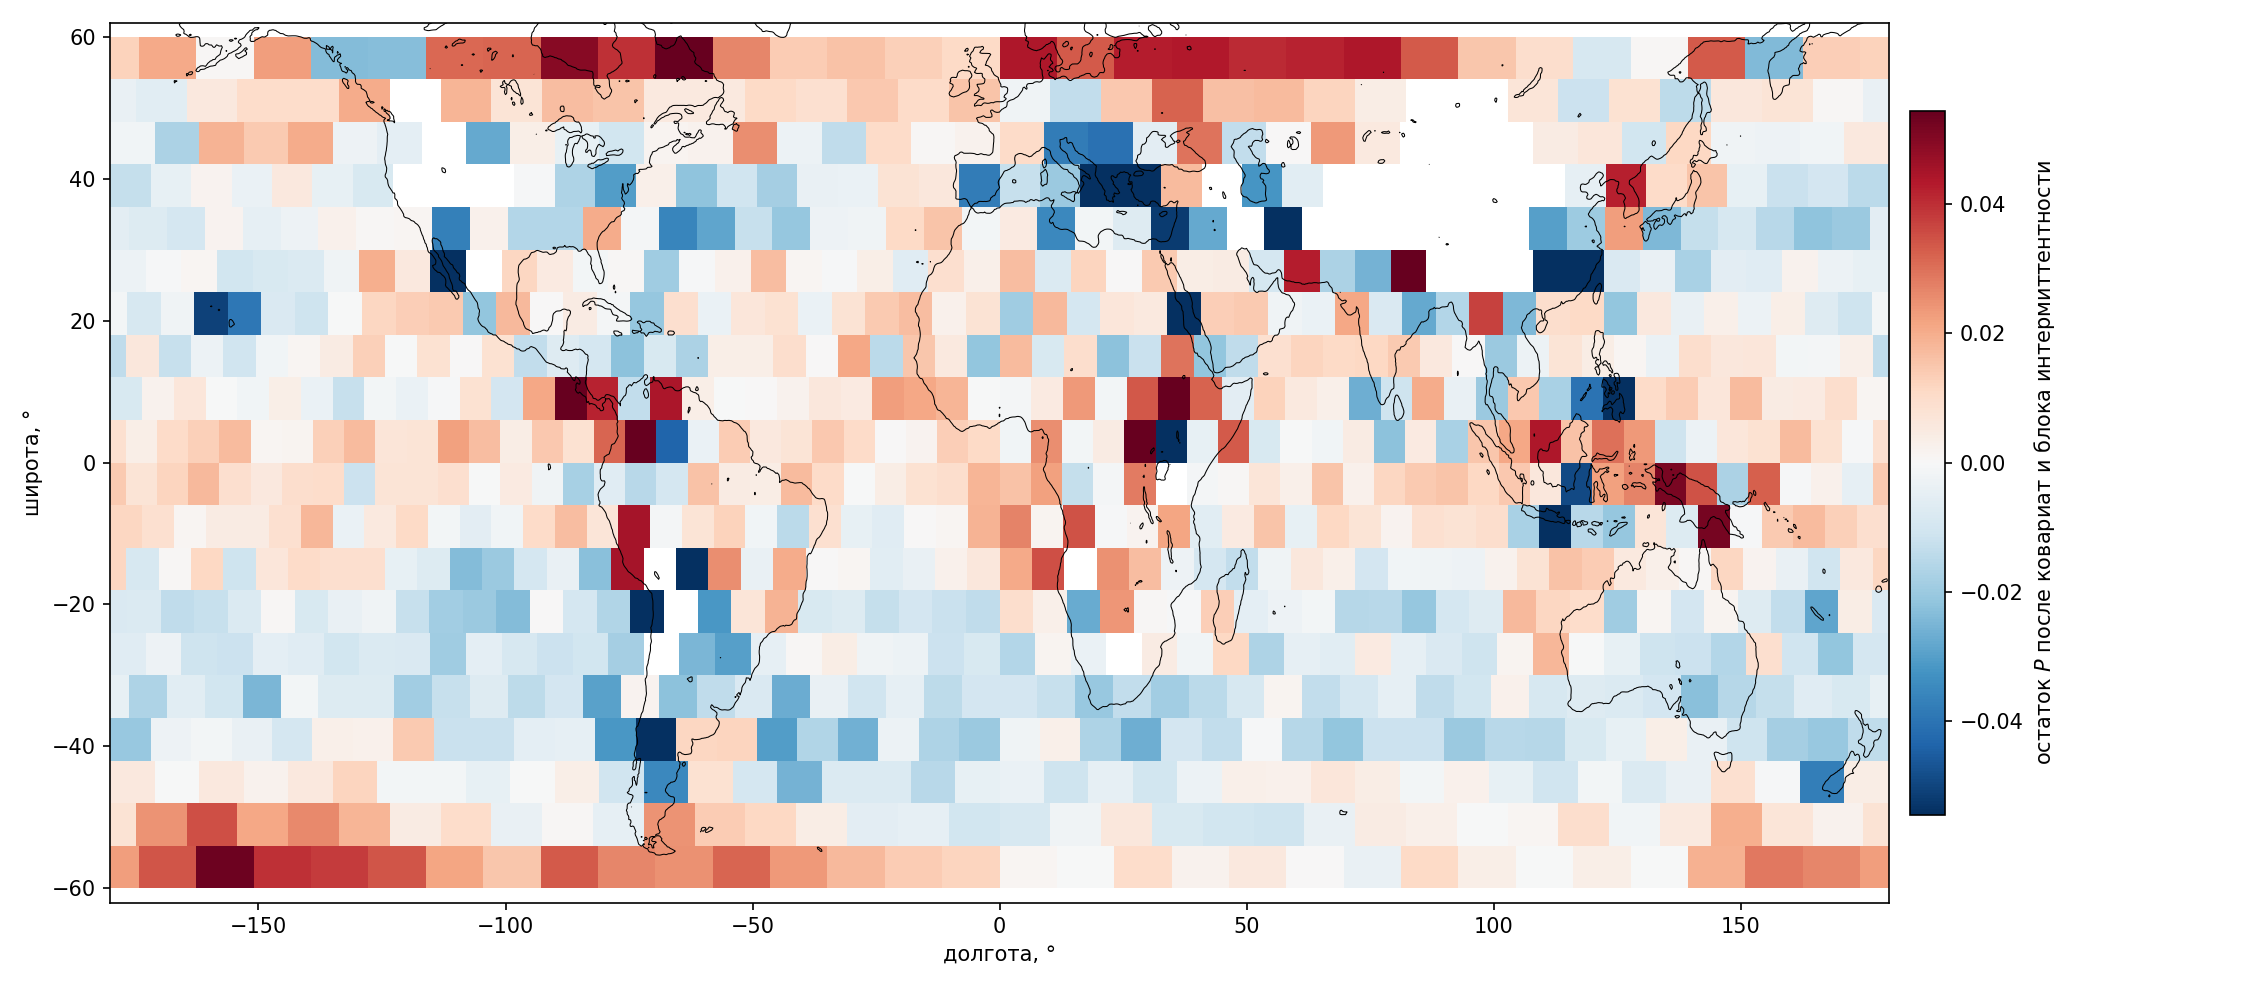
\includegraphics[width=\linewidth]{figures/fig3_residual_map.png}
\caption{Остаток глобальной карты $P$ после восьми ковариат атрибуции и блока статистик интермиттентности (среднее двух сезонов 2023~г.; регрессия обучена на противоположной временной половине выборки, поэтому остаток свободен от общего выборочного шума). Синие доли --- сопряжённость ниже предсказанной (муссонные окраины, склоны орографии), красные --- выше (очаги глубокой конвекции, высокоширотные окраины суши). Белым --- тайлы, исключённые по орографии.}
\label{fig:residual}
\end{figure}

\section{Проверка следствия статичности и границы применимости}
\label{sec:bounds}

\emph{Прямая проверка следствия.} Если $P$ --- статичный функционал сложившегося режима, он по определению не должен опережать перестройку режима и превосходить по чувствительности стандартные показатели. На единственном крупном документированном переходе внутри записи --- сдвиге Междекадного тихоокеанского колебания 1998/99~гг. --- доля случаев, в которых статистика перехода $P$ опережает конкурента, составила 25\,\% против CAPE, 47\,\% против синоптической вихревой энергии и 42\,\% против наклона спектра при пороге опережающего поведения 60\,\%; по медианному отношению <<сигнал/шум>> многолетнего тренда $P$ занимает последнее место из четырёх показателей (0,67 против 2,39 у CAPE). Это \emph{подтверждение} исходной гипотезы, а не отклонённое применение: величина ведёт себя ровно так, как обязана вести себя статичная проекция инвариантной меры, и в таком виде результат зафиксирован также в статье~II.

\emph{Отдельно и честно открытый вопрос --- устойчивость самого $\theta(x)$.} В тайлах наибольшего многолетнего тренда CAPE обнаружен слабый отрицательный тренд спектрально-фиксированного $P$ ($-8{,}5\cdot10^{-5}$~год$^{-1}$, $p=0{,}025$, доверительный интервал кластерного бутстрэпа исключает ноль), однако единственный доступный свободный расчёт с переходным форсингом воспроизводит его лишь на $\sim$27\,\% величины и статистически неотличимо от нуля ($p=0{,}22$). Это вопрос о том, не начало ли квенчированное поле условий смещаться на человеческом горизонте --- возможность, которую рамка допускает вдоль расширяющихся конвективных окраин, --- а не о динамике $P$ как переменной. Статья не разрешает этот вопрос и оставляет его открытым: внутри одного реанализа, охватывающего крупные смены наблюдательной системы, факт тренда не отделим от инструментального дрейфа.

\emph{Граница применимости рамки} устанавливается явно. Статья не делает и не подразумевает: количественных предсказаний динамики режима на основе $P$ (первый пункт этого раздела фиксирует прямо противоположное); вариационного или динамического вывода наблюдаемой из первых принципов (такой вывод не проводился и не заявляется); каких-либо приложений за пределами географии и статистики циркуляции. Сведение $P$ к стандартным наблюдаемым инвариантной меры (локальная размерность, экстремальный индекс, спектр оператора переноса) остаётся незавершённым направлением: предварительный пилот ($\rho(P,d)\approx+0{,}5$ на 48 оконных выборках) фиксирует содержательность вопроса, но не его решение.

\section{Выводы}
\label{sec:conclusion}

1.~Аудит новизны конструкции завершён: сопряжённость соседних огибающих масштабных полос --- известная форма оценки, ближайшие родственники которой --- корреляция амплитудных огибающих в нейрофизиологии и коэффициент амплитудной модуляции в турбулентности; рангово-копульная составляющая декоративна ($\rho=0{,}99$ с линейным аналогом). Новизна серии --- в свойствах объекта: устойчивости, физической атрибутируемости, воспроизводимости без усвоения наблюдений, --- а не в оценивающей статистике.

2.~Запись $P(x)=\Phi[\mu_{\theta(x)}]$ формализует статус инварианта как функционала стационарной меры быстрого слоя при квенчированном поле условий $\theta(x)$ ($T_{\mathrm{fast}}\approx10$~ч против $T_\theta\gg46$~лет). Отсутствие у такого функционала собственной динамики --- не постулат, а трижды независимо подтверждённый отрицательный результат (релаксация, плоская иерархия времён, тождество для класса оценщиков производной).

3.~Интерпретирующий язык статьи не выходит за пределы измеренного: без утверждений об активной связи между масштабами, без динамического или вариационного вывода, без решённых модельных примеров сверх приведённых; ни одно из этих ограничений в настоящей статье не снимается и не выдаётся за снятое.

4.~Практическая ценность инварианта --- районирование: многомерное (не менее одиннадцати осей) поле локальных условий проецируется на устойчивую скалярную ось, эффективно одномерную (одна ковариата --- 85\,\% качества предсказания); необъяснённые $\approx$15\,\% воспроизводимой дисперсии карты --- воспроизводимая, географически организованная, но не идентифицированная структура, отнесённая к дальнейшей работе.

5.~Прямая проверка следствия статичности (переход 1998/99~гг.) подтверждает гипотезу: инвариант не опережает и не превосходит по чувствительности стандартные показатели при перестройке режима --- ожидаемое, а не аномальное поведение статичной проекции. Вопрос об устойчивости самого поля условий $\theta(x)$ на многодесятилетнем горизонте остаётся отдельным и открытым.

6.~Статья не делает выводов за пределами описанной рамки: рамка предлагается как основание для дальнейшей эмпирической, географической и статистической работы --- в первую очередь по идентификации источников остаточной географии и по включению $P$ в практические схемы районирования, --- а не как завершённая теория.

\paragraph{Данные и код.} Все протоколы (включая четыре аудита новизны и надёжности), программный код и численные результаты открыты в репозитории: \url{https://github.com/Theclimateguy/Shroedinger}.

\printbibliography[title={Список литературы}]

\end{document}
